% =============================================================================
%  Machine Learning for Petroleum Engineers Using Python
%  Módulo 7 · Clase 2: El Tasador --- Un Modelo de Punta a Punta
%  SLB Ecuador | UDLA
%
%  Compilar: pdflatex -shell-escape presentacion.tex (x2 para refs)
% =============================================================================
\documentclass[aspectratio=169, 11pt]{beamer}

% ── Codificación y lenguaje ──────────────────────────────────────────────────
\usepackage[T1]{fontenc}
\usepackage[utf8]{inputenc}
\usepackage[spanish,es-noshorthands]{babel}

% ── Fuentes ──────────────────────────────────────────────────────────────────
\usepackage{FiraSans}
\usepackage{FiraMono}
\renewcommand{\familydefault}{\sfdefault}

% ── Gráficos y diagramas ────────────────────────────────────────────────────
\usepackage{graphicx}
\usepackage{tikz}
\usetikzlibrary{arrows.meta, positioning, shapes.geometric, calc, fit, decorations.pathreplacing}
\usepackage{fontawesome5}

% ── Código fuente ────────────────────────────────────────────────────────────
\usepackage{minted}
\usepackage{tcolorbox}
\tcbuselibrary{minted, skins, breakable}

% ── Tablas y utilidades ──────────────────────────────────────────────────────
\usepackage{amsmath}
\usepackage{colortbl}
\usepackage{booktabs}
\usepackage{multicol}
\usepackage{hyperref}
\usepackage{calc}

% =============================================================================
%  PALETA DE COLORES (rojo UDLA + variantes)
% =============================================================================
\definecolor{arcaRed}{HTML}{C82B40}
\definecolor{arcaDark}{HTML}{6B1525}
\definecolor{udlaCrimson}{HTML}{A31545}
\definecolor{arcaGray}{HTML}{F5F5F5}
\definecolor{arcaLightGray}{HTML}{EBEBEB}
\definecolor{textDark}{HTML}{2D2D2D}
\definecolor{textMuted}{HTML}{6B7280}
\definecolor{codeGreen}{HTML}{16A34A}
\definecolor{codeBlue}{HTML}{2563EB}
\definecolor{codeOrange}{HTML}{EA580C}
\definecolor{slbBlue}{HTML}{0014DC}
\definecolor{terminalBg}{HTML}{0F172A}
\definecolor{terminalGreen}{HTML}{86EFAC}
\definecolor{terminalMuted}{HTML}{94A3B8}
\definecolor{codeBg}{HTML}{FAFAFA}

% =============================================================================
%  CONFIGURACIÓN DEL TEMA BEAMER
% =============================================================================
\usetheme{default}
\usecolortheme{default}

\setbeamertemplate{navigation symbols}{}
\setbeamertemplate{footline}{}
\setbeamertemplate{headline}{}

\setbeamercolor{normal text}{fg=textDark}
\setbeamercolor{frametitle}{fg=arcaRed, bg=white}
\setbeamercolor{title}{fg=white}
\setbeamercolor{subtitle}{fg=white!85}
\setbeamercolor{author}{fg=white!80}
\setbeamercolor{date}{fg=white!70}
\setbeamercolor{item}{fg=arcaRed}
\setbeamercolor{subitem}{fg=arcaDark}
\setbeamercolor{block title}{fg=white, bg=arcaRed}
\setbeamercolor{block body}{fg=textDark, bg=arcaGray}
\setbeamercolor{block title alerted}{fg=white, bg=codeOrange}
\setbeamercolor{block body alerted}{fg=textDark, bg=arcaGray}
\setbeamercolor{block title example}{fg=white, bg=codeGreen}
\setbeamercolor{block body example}{fg=textDark, bg=arcaGray}
\setbeamercolor{section in toc}{fg=arcaDark}

\setbeamerfont{frametitle}{size=\Large, series=\bfseries}
\setbeamerfont{title}{size=\huge, series=\bfseries}
\setbeamerfont{subtitle}{size=\large}
\setbeamerfont{author}{size=\normalsize}
\setbeamerfont{date}{size=\small}
\setbeamerfont{block title}{size=\normalsize, series=\bfseries}
\setbeamerfont{footnote}{size=\tiny}

\setbeamertemplate{itemize item}{\scriptsize\raise1.5pt\hbox{\color{arcaRed}$\blacktriangleright$}}
\setbeamertemplate{itemize subitem}{\scriptsize\raise1pt\hbox{\color{arcaDark}$\bullet$}}
\setbeamertemplate{enumerate items}[default]
\setbeamercolor{enumerate item}{fg=arcaRed}

% =============================================================================
%  HEADER
% =============================================================================
\setbeamertemplate{headline}{%
  \begin{tikzpicture}[remember picture, overlay]
    \fill[arcaDark] (current page.north west) rectangle
      ([yshift=-0.7cm]current page.north east);
    \node[anchor=west, inner sep=0pt] at
      ([xshift=0.6cm, yshift=-0.35cm]current page.north west)
      {
\includegraphics[height=0.45cm]{../logo_udla_white.png}};
    \node[anchor=east, inner sep=0pt] at
      ([xshift=-0.6cm, yshift=-0.35cm]current page.north east)
      {
\includegraphics[height=0.42cm]{../SLB_white.png}};
  \end{tikzpicture}%
  \vspace{0.7cm}%
}

% =============================================================================
%  FOOTER
% =============================================================================
\setbeamertemplate{footline}{%
  \begin{tikzpicture}[remember picture, overlay]
    \draw[arcaLightGray, line width=0.4pt]
      ([yshift=0.55cm, xshift=0.6cm]current page.south west) --
      ([yshift=0.55cm, xshift=-0.6cm]current page.south east);
    \node[anchor=south, font=\tiny\color{textMuted}] at
      ([yshift=0.15cm]current page.south)
      {Machine Learning for Petroleum Engineers Using Python \(\cdot\) SLB Ecuador};
    \node[anchor=south east, font=\scriptsize\bfseries\color{arcaRed}] at
      ([xshift=-0.6cm, yshift=0.15cm]current page.south east)
      {\insertframenumber};
  \end{tikzpicture}%
}

% =============================================================================
%  FRAMETITLE personalizado con línea roja
% =============================================================================
\setbeamertemplate{frametitle}{%
  \vspace{0.25cm}%
  \usebeamerfont{frametitle}\usebeamercolor[fg]{frametitle}\insertframetitle%
  \par\vspace{2pt}%
  \begin{tikzpicture}
    \fill[arcaRed] (0,0) rectangle (3cm, 1.5pt);
    \fill[arcaLightGray] (3cm,0) rectangle (\textwidth, 0.5pt);
  \end{tikzpicture}%
  \vspace{0.1cm}%
}

% =============================================================================
%  ESTILO DE BLOQUES DE CÓDIGO (minted + tcolorbox)
% =============================================================================
\newtcblisting{pyblock}[1][]{%
  listing engine=minted,
  minted language=python,
  minted style=xcode,
  minted options={
    fontsize=\small,
    linenos=false,
    breaklines=true,
    python3=true
  },
  enhanced,
  colback=codeBg,
  colframe=arcaRed,
  left=8pt,
  right=6pt,
  top=5pt,
  bottom=5pt,
  boxrule=0pt,
  leftrule=3pt,
  arc=3pt,
  listing only,
  title={\hspace{-2pt}\faPython\hspace{5pt}Python},
  fonttitle=\scriptsize\bfseries,
  colbacktitle=arcaRed,
  coltitle=white,
  attach boxed title to top left={xshift=8pt, yshift=-7pt},
  boxed title style={
    arc=2pt, boxrule=0pt,
    top=1.5pt, bottom=1.5pt, left=6pt, right=6pt
  },
  drop fuzzy shadow=black!12,
  #1
}

\newtcblisting{outputblock}[1][]{%
  listing engine=minted,
  minted language=text,
  minted style=bw,
  minted options={
    fontsize=\small,
    breaklines=true,
    formatcom=\color{terminalGreen}
  },
  enhanced,
  colback=terminalBg,
  colframe=terminalBg,
  coltext=terminalGreen,
  left=10pt, right=6pt, top=5pt, bottom=5pt,
  boxrule=0pt,
  arc=3pt,
  listing only,
  title={\hspace{-2pt}\faTerminal\hspace{5pt}Output},
  fonttitle=\scriptsize\bfseries,
  colbacktitle=terminalGreen!85!black,
  coltitle=terminalBg,
  attach boxed title to top left={xshift=8pt, yshift=-7pt},
  boxed title style={
    arc=2pt, boxrule=0pt,
    top=1.5pt, bottom=1.5pt, left=6pt, right=6pt
  },
  #1
}

% =============================================================================
%  SECTION DIVIDERS
% =============================================================================
\newcommand{\sectionframe}[2]{%
  \begingroup
    \setbeamertemplate{headline}{}
    \setbeamertemplate{footline}{}
    \setbeamertemplate{navigation symbols}{}
    \begin{frame}[plain, noframenumbering]
      \begin{tikzpicture}[remember picture, overlay]
        \fill[arcaRed] (current page.south west) rectangle (current page.north east);
        \node[anchor=center, text=white, font=\Huge\bfseries, text width=15cm,
              align=center] at ([yshift=0.5cm]current page.center)
              {\hyphenpenalty=10000\exhyphenpenalty=10000 #1};
        \node[anchor=center, text=white!80, font=\large, text width=10cm,
              align=center] at ([yshift=-0.8cm]current page.center) {#2};
      \end{tikzpicture}
    \end{frame}
  \endgroup
}

% =============================================================================
%  METADATOS
% =============================================================================
\title{Machine Learning for Petroleum Engineers\\Using Python}
\subtitle{Módulo 7 · Clase 2: El Tasador --- Un Modelo de Punta a Punta}
\author{Carlos Enrique Mosquera Trujillo}
\date{2026}

% =============================================================================
%  DOCUMENTO
% =============================================================================
% =============================================================================
%  DOCUMENTO
% =============================================================================
% =============================================================================
%  Cajas de PROMPT (demo: se copian al agente) y de ENCARGO (retos: sin
%  solucion en ninguna parte del material).
% =============================================================================
\newtcolorbox{prompt}[1][]{%
  colback=arcaGray, colframe=arcaDark, boxrule=0pt, leftrule=3.5pt,
  arc=3pt, left=8pt, right=8pt, top=6pt, bottom=6pt,
  fontupper=\ttfamily\scriptsize\color{textMuted},
  title={\hspace{-2pt}\faRobot\hspace{5pt}#1},
  fonttitle=\scriptsize\bfseries\sffamily,
  colbacktitle=arcaDark, coltitle=white,
  attach boxed title to top left={xshift=8pt, yshift=-7pt},
  boxed title style={arc=2pt, boxrule=0pt,
    top=1.5pt, bottom=1.5pt, left=6pt, right=6pt}}

\newtcolorbox{encargo}[1][]{%
  colback=white, colframe=arcaRed, boxrule=1.4pt,
  arc=3pt, left=8pt, right=8pt, top=5pt, bottom=5pt,
  title={\hspace{-2pt}\faTools\hspace{5pt}#1},
  fonttitle=\scriptsize\bfseries\sffamily,
  colbacktitle=arcaRed, coltitle=white,
  attach boxed title to top left={xshift=8pt, yshift=-7pt},
  boxed title style={arc=2pt, boxrule=0pt,
    top=1.5pt, bottom=1.5pt, left=6pt, right=6pt}}

\begin{document}
% ── PORTADA ──────────────────────────────────────────────────────────────────
{
\setbeamertemplate{headline}{}
\setbeamertemplate{footline}{}
\begin{frame}[plain, noframenumbering]
  \begin{tikzpicture}[remember picture, overlay]
    \fill[white] (current page.south west) rectangle (current page.north east);
    \fill[arcaRed] (current page.north west) rectangle ([yshift=-0.35cm]current page.north east);
    \fill[arcaDark] (current page.south west) rectangle ([yshift=0.35cm]current page.south east);
    \fill[arcaRed]
      ([xshift=1.1cm, yshift=-0.35cm]current page.north west) rectangle
      ([xshift=1.15cm, yshift=0.35cm]current page.south west);
    \node[anchor=north west, inner sep=0pt] at
      ([xshift=1.8cm, yshift=-1.2cm]current page.north west)
      {
\includegraphics[height=1.6cm]{../logo_udla.png}};
    \node[anchor=north east, inner sep=0pt] at
      ([xshift=-1.5cm, yshift=-1.2cm]current page.north east)
      {
\includegraphics[height=1.5cm]{../SLB.png}};
    \node[anchor=center, text=arcaDark, text width=14.5cm, align=center] at
      ([yshift=0.95cm]current page.center) {
        {\LARGE\bfseries Machine Learning for Petroleum Engineers}\\[8pt]
        {\LARGE\bfseries Using Python}
      };
    \fill[arcaRed]
      ([yshift=-0.35cm, xshift=-3.2cm]current page.center) rectangle
      ([yshift=-0.28cm, xshift=3.2cm]current page.center);
    \node[anchor=center, text=arcaRed, font=\large, text width=13cm, align=center] at
      ([yshift=-1.3cm]current page.center) {
        Módulo 7 · Clase 2\\[3pt]
        El Tasador --- Un Modelo de Punta a Punta
      };
    \node[anchor=center, text=textMuted, font=\normalsize] at
      ([yshift=-2.5cm]current page.center) {
        {\color{arcaRed}\faUser}\hspace{6pt}Carlos Enrique Mosquera Trujillo
        \hspace{16pt}
        {\color{arcaRed}\faIndustry}\hspace{4pt}SLB Ecuador
      };
  \end{tikzpicture}
\end{frame}
}

% ── DÓNDE ESTAMOS ────────────────────────────────────────────────────────────
\begin{frame}[shrink=5]{Dónde Estamos: Hoy se Paga lo Pendiente}
  \vspace{-2pt}
  \begin{columns}[T]
    \begin{column}{0.48\textwidth}
      {\small\color{arcaDark}\bfseries\faCheckCircle\hspace{5pt}De la Clase 1 ya tienen:}
      \vspace{4pt}
      {\footnotesize\color{textMuted}
      \begin{itemize}\setlength{\itemsep}{4pt}
        \item[{\color{codeGreen}\scriptsize\faCheck}]
          Los \textbf{cuatro fundamentos} de un encargo: objetivo, contexto,
          restricciones, criterio de aceptación
        \item[{\color{codeGreen}\scriptsize\faCheck}]
          Gráficas que se defienden solas
        \item[{\color{codeGreen}\scriptsize\faCheck}]
          La regla del cero: un cero perfecto casi siempre es una
          \textbf{ausencia}
      \end{itemize}}
      \vspace{4pt}
      {\scriptsize\color{textMuted}\itshape
       Y quedó pendiente la app con link --- el tiempo no alcanzó. Hoy se
       paga, y con intereses.}
    \end{column}
    \begin{column}{0.48\textwidth}
      {\small\color{arcaDark}\bfseries\faForward\hspace{5pt}Hoy:}
      \vspace{4pt}
      {\footnotesize\color{textMuted}
      \begin{itemize}\setlength{\itemsep}{4pt}
        \item[{\color{arcaRed}\scriptsize\faArrowRight}]
          \textbf{Un modelo de punta a punta}, con un solo caso de inicio a
          fin: el tasador de diamantes
        \item[{\color{arcaRed}\scriptsize\faArrowRight}]
          Certificar $\to$ entrenar $\to$ examinar $\to$ guardar $\to$
          \textbf{servir} $\to$ blindar
        \item[{\color{arcaRed}\scriptsize\faStar}]
          Y el mismo flujo, \textbf{hecho por ustedes} en otro caso ---
          que es la pieza central de su proyecto
      \end{itemize}}
    \end{column}
  \end{columns}
  \vspace{4pt}
  {\scriptsize\color{arcaDark}\itshape
   Recordatorio del proyecto: equipos de hasta 3, entrega hasta el jueves de
   la próxima semana. Lo de hoy es exactamente lo que su proyecto necesita.}
\end{frame}

% ── EL CASO ──────────────────────────────────────────────────────────────────
\begin{frame}[shrink=5]{El Caso · El Comprador de Diamantes}
  \vspace{-2pt}
  \begin{columns}[T]
    \begin{column}{0.47\textwidth}
      \begin{tcolorbox}[colback=arcaGray, colframe=arcaRed, boxrule=0pt,
        leftrule=3pt, arc=3pt, left=7pt, right=7pt, top=3pt, bottom=3pt]
        {\scriptsize\color{arcaRed}\bfseries EL PROBLEMA}\\[2pt]
        {\scriptsize\color{textMuted}
         Su cliente compra lotes de piedras. Hoy tasa \textbf{a ojo y por
         comparables}, piedra por piedra: lento, y depende de quién tasa
         ese día.}
      \end{tcolorbox}
      \vspace{2pt}
      \begin{tcolorbox}[colback=arcaGray, colframe=arcaDark, boxrule=0pt,
        leftrule=3pt, arc=3pt, left=7pt, right=7pt, top=3pt, bottom=3pt]
        {\scriptsize\color{arcaDark}\bfseries LA DECISIÓN}\\[2pt]
        {\scriptsize\color{textMuted}
         Frente a cada piedra: \textbf{comprar o pasar}, y a qué precio
         máximo. Cientos de veces por lote.}
      \end{tcolorbox}
    \end{column}
    \begin{column}{0.47\textwidth}
      \begin{tcolorbox}[colback=arcaGray, colframe=arcaDark, boxrule=0pt,
        leftrule=3pt, arc=3pt, left=7pt, right=7pt, top=3pt, bottom=3pt]
        {\scriptsize\color{arcaDark}\bfseries EL COSTO DEL ERROR}\\[2pt]
        {\scriptsize\color{textMuted}
         Comprar caro \textbf{no se nota hasta vender}. Y pasar de largo una
         piedra buena es margen regalado al competidor.}
      \end{tcolorbox}
      \vspace{2pt}
      \begin{tcolorbox}[colback=arcaGray, colframe=codeGreen, boxrule=0pt,
        leftrule=3pt, arc=3pt, left=7pt, right=7pt, top=3pt, bottom=3pt]
        {\scriptsize\color{codeGreen}\bfseries QUÉ NOS PIDIÓ}\\[2pt]
        {\scriptsize\color{textMuted}
         «Un \textbf{tasador}: le meto las medidas de la piedra y me dice
         cuánto vale. Que lo use mi gente en la mesa de compra, sin
         llamarlos a ustedes.»}
      \end{tcolorbox}
    \end{column}
  \end{columns}
  \vspace{2pt}
  {\scriptsize\color{arcaDark}\bfseries
   Tiene 53.940 compras históricas con precio pagado. Eso es todo lo que
   hace falta para intentarlo.}
\end{frame}
\begin{frame}[shrink=5]{Ustedes Ya Hacen Esto}
  \vspace{4pt}
  {\footnotesize\color{textMuted}
   ¿Cómo tasa hoy el comprador, sin modelo? \textbf{Por comparables}: busca
   en su memoria piedras parecidas que ya compró, y ajusta por las
   diferencias.
   \vspace{6pt}

   Eso es \emph{exactamente} lo que hicieron en el Módulo 5 con las
   reservas: los \textbf{análogos} --- «de los campos que estuvieron donde
   está el mío, ¿dónde terminaron?».}
  \vspace{7pt}
  \begin{tcolorbox}[colback=arcaGray, colframe=arcaDark, boxrule=0pt,
    leftrule=4pt, arc=3pt, left=10pt, right=10pt, top=6pt, bottom=6pt]
    {\footnotesize\color{arcaDark}\bfseries
     Un modelo de precios es la memoria de comparables del comprador ---
     pero con 53.940 casos en vez de los cientos que caben en una cabeza,
     y disponible para todo su equipo a la vez.}
  \end{tcolorbox}
  \vspace{7pt}
  {\footnotesize\color{arcaDark}\itshape
   No estamos reemplazando su criterio: estamos poniendo su manera de
   pensar dentro de una herramienta que no se cansa ni se enferma.}
\end{frame}


\begin{frame}[shrink=5]{El Mapa de la Clase: Seis Pasos, Un Flujo}
  \vspace{4pt}
  \begin{center}
  \begin{tikzpicture}[
    caja/.style={draw, rounded corners=2pt, line width=1.1pt, align=center,
                 minimum height=0.88cm, minimum width=1.72cm,
                 font=\tiny\bfseries},
    sub/.style={font=\tiny, text=textMuted, align=center},
    fl/.style={-{Stealth[length=2mm]}, line width=1pt, color=gray}]
    \node[caja, color=arcaRed]   (a) at (0,0)     {1\\CERTIFICAR};
    \node[caja, color=arcaDark]  (b) at (2.06,0)  {2\\ENTRENAR};
    \node[caja, color=arcaDark]  (c) at (4.12,0)  {3\\EXAMINAR};
    \node[caja, color=arcaDark]  (d) at (6.18,0)  {4\\GUARDAR};
    \node[caja, color=blue!60!black] (e) at (8.24,0) {5\\SERVIR};
    \node[caja, color=codeGreen] (f) at (10.3,0)  {6\\BLINDAR};
    \draw[fl] (a) -- (b); \draw[fl] (b) -- (c); \draw[fl] (c) -- (d);
    \draw[fl] (d) -- (e); \draw[fl] (e) -- (f);
    \node[sub] at (0,-0.75)    {¿el dato\\es real?};
    \node[sub] at (2.06,-0.75) {el bosque\\aprende};
    \node[sub] at (4.12,-0.75) {con piedras\\que no vio};
    \node[sub] at (6.18,-0.75) {el modelo es\\un archivo};
    \node[sub] at (8.24,-0.75) {la app\\con link};
    \node[sub] at (10.3,-0.75) {que no\\mienta};
  \end{tikzpicture}
  \end{center}
  \vspace{6pt}
  {\footnotesize\color{textMuted}
   Este es \textbf{el flujo completo de un producto de datos} --- el mismo en
   cualquier empresa, con cualquier herramienta. Hoy lo recorremos entero una
   vez conmigo, y una vez ustedes.}
  \vspace{5pt}

  {\footnotesize\color{arcaDark}\bfseries\itshape
   Fíjense dónde empieza: no en el modelo. En preguntarle al dato si dice la
   verdad. Eso ya lo saben hacer desde la Clase 1.}
\end{frame}

% ═════════════════════════════════════════════════════════════════════════════
\sectionframe{Paso 1 · Certificar}{Nadie entrena con datos que no revisó \\[6pt] \normalsize 12 -- 28 min}
% ═════════════════════════════════════════════════════════════════════════════

\begin{frame}[shrink=5]{Recorderis de la Clase 1: el Cero que No Es Cero}
  \vspace{2pt}
  {\scriptsize\color{textMuted}
   En la Clase 1 vimos 1.812 viajes en efectivo con \textbf{exactamente
   cero} propinas --- y la conclusión fácil era falsa: el taxímetro no
   registra la propina en efectivo. Un cero que era una \textbf{ausencia}.
   \vspace{2pt}

   La regla que salió de ahí: en datos reales, \textbf{nada es exactamente
   cero por casualidad}. Y hoy la aplicamos antes de entrenar nada.}
  \vspace{2pt}
  \begin{prompt}[EL PROMPT DE LA DEMO --- la revisión, antes que el modelo]
Voy a entrenar un modelo de precios con el DataFrame
`diamantes` (53.940 filas). Columnas: carat, cut,
color, clarity, price [USD], y x, y, z que son las
dimensiones físicas de la piedra en milímetros.

ANTES de cualquier modelo: revisión de calidad.
- mínimo, máximo y ceros de cada columna numérica
- dime si algún valor es FÍSICAMENTE imposible para
  un diamante (pista: son milímetros)
- cuántas filas afectadas, y muéstramelas
  \end{prompt}
  \vspace{2pt}
  {\scriptsize\color{arcaDark}\itshape
   El mismo prompt de revisión de la Clase 1, afinado al caso. Ya es de
   ustedes: se corre antes de cada análisis, siempre.}
\end{frame}

\begin{frame}[shrink=8]{Lo que Aparece: 23 Piedras que No Existen}
  \vspace{-2pt}
  \begin{center}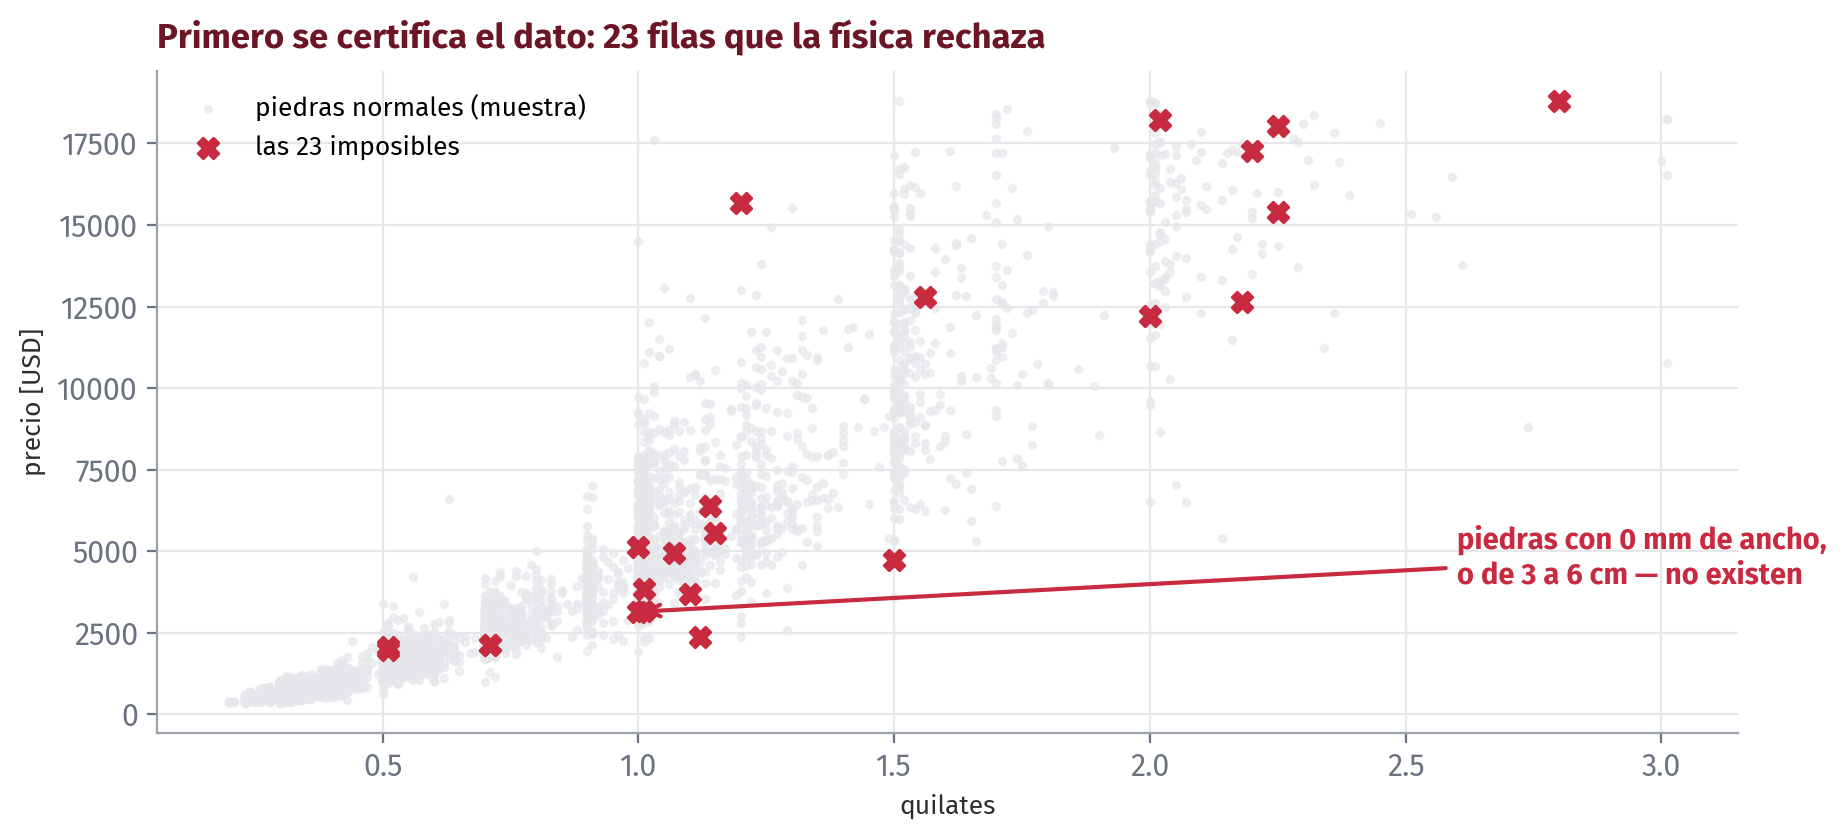
\includegraphics[width=0.92\textwidth, height=0.46\textheight, keepaspectratio]{fig_certificar.png}\end{center}
  \vspace{2pt}
  {\footnotesize\color{textMuted}
   Piedras con \textbf{0 mm} de alguna dimensión --- no existen --- y un par
   con 3 a 6 \textbf{centímetros}, que serían piedras de museo a precio de
   anillo. Errores de captura, no diamantes.}
\end{frame}

\begin{frame}[shrink=5]{La Decisión de Certificación}
  \vspace{4pt}
  {\footnotesize\color{textMuted}
   ¿Qué se hace con 23 filas malas entre 53.940? La decisión tiene tres
   partes, y las tres se \textbf{escriben}:}
  \vspace{6pt}
  {\footnotesize\color{textMuted}
  \begin{enumerate}\setlength{\itemsep}{6pt}
    \item \textbf{Se rechazan} las 23 --- con argumento físico, no estético:
          una dimensión de 0 mm no es una piedra, es un campo vacío
          disfrazado de número.
    \item \textbf{Se le avisa al dueño del dato}, en dos frases: qué se
          encontró y qué se hizo. Hoy son 23 inofensivas; mañana pueden ser
          las 5.000 que cambian el negocio.
    \item \textbf{Queda registrado en el código}: el filtro con su
          comentario. El que herede esto sabrá qué se quitó y por qué.
  \end{enumerate}}
  \vspace{7pt}
  \begin{tcolorbox}[colback=arcaGray, colframe=arcaDark, boxrule=0pt,
    leftrule=4pt, arc=3pt, left=9pt, right=9pt, top=5pt, bottom=5pt]
    {\footnotesize\color{arcaDark}\bfseries
     Quedan 53.917 piedras certificadas. Recién ahora se puede entrenar.}
  \end{tcolorbox}
\end{frame}

% ═════════════════════════════════════════════════════════════════════════════
\sectionframe{Pasos 2 y 3 · Entrenar y Examinar}{El bosque aprende, y rinde examen con piedras que no vio \\[6pt] \normalsize 28 -- 50 min}
% ═════════════════════════════════════════════════════════════════════════════

\begin{frame}[shrink=5]{Recorderis: Qué Es Entrenar un Modelo}
  \vspace{2pt}
  {\scriptsize\color{textMuted}
   Lo vieron en el Módulo 5, y como acá nada se da por sabido, en una frase:}
  \vspace{2pt}
  \begin{tcolorbox}[colback=arcaGray, colframe=arcaDark, boxrule=0pt,
    leftrule=4pt, arc=3pt, left=10pt, right=10pt, top=3pt, bottom=3pt]
    {\scriptsize\color{arcaDark}\bfseries
     Entrenar es mostrarle al modelo miles de casos que ya terminaron ---
     piedra, medidas, y \emph{lo que de verdad se pagó} --- hasta que
     aprende la relación entre las medidas y el precio.}
  \end{tcolorbox}
  \vspace{2pt}
  {\scriptsize\color{textMuted}
   Usamos el \textbf{Random Forest} --- el bosque de las clases del Módulo 5:
   cien árboles de decisión, cada uno aprende de una muestra distinta, y la
   tasación es el voto de todos.
   \vspace{2pt}

   Y la regla de oro del examen, que también ya conocen: se \textbf{reserva
   el 20\,\%} de las piedras \emph{antes} de entrenar. El modelo jamás las
   ve. Con esas se le toma el examen --- porque examinarlo con piedras que
   memorizó es hacerle trampa a favor.}
  \vspace{2pt}
  {\scriptsize\color{arcaDark}\itshape
   ¿Por qué no un modelo más moderno y complicado? Porque primero se mide si
   el simple alcanza. Es la regla del récord a batir, de todo el diplomado.}
\end{frame}

\begin{frame}[fragile, shrink=5]{Desde Cero: el Modelo No Come Texto}
  \vspace{2pt}
  {\footnotesize\color{textMuted}
   El corte de una piedra es \texttt{"Ideal"} o \texttt{"Premium"} ---
   palabras. Y un modelo solo sabe de números. La conversión estándar se
   llama \texttt{get\_dummies}: cada categoría se vuelve una columna de
   unos y ceros.}
  \vspace{5pt}
  \begin{minted}[fontsize=\scriptsize, breaklines]{python}
pd.get_dummies(d[["carat", "cut"]], columns=["cut"])
#  carat  cut_Fair  cut_Good  cut_Ideal  cut_Premium ...
#   0.23         0         0          1            0
#   0.21         0         0          0            1
  \end{minted}
  \vspace{5pt}
  {\footnotesize\color{textMuted}
   La piedra \texttt{Ideal} tiene un 1 en su columna y 0 en las demás. Nada
   más que eso.}
  \vspace{5pt}
  \begin{tcolorbox}[colback=arcaGray, colframe=arcaRed, boxrule=0pt,
    leftrule=3pt, arc=3pt, left=8pt, right=8pt, top=4pt, bottom=4pt]
    {\scriptsize\color{arcaRed}\bfseries GUARDEN ESTE DETALLE}\\[2pt]
    {\footnotesize\color{textMuted}
     Esta conversión crea \textbf{muchas columnas nuevas, en un orden}. La
     app va a tener que reproducir \emph{exactamente} las mismas columnas en
     \emph{exactamente} el mismo orden. Vuelve en un rato --- y muerde.}
  \end{tcolorbox}
\end{frame}

\begin{frame}[shrink=5]{El Encargo de Entrenamiento}
  \vspace{2pt}
  \begin{prompt}[EL PROMPT DE LA DEMO --- entrenar y examinar]
Con el DataFrame `d` ya certificado (53.917 piedras):

OBJETIVO: un modelo que estime el precio [USD] a
partir de carat, cut, color, clarity, x, y, z,
depth y table.

RESTRICCIONES:
- RandomForestRegressor de scikit-learn, 100 árboles,
  random_state=0
- reserva el 20% para examen ANTES de entrenar
  (train_test_split, random_state=0)
- las columnas de texto (cut, color, clarity)
  conviértelas con get_dummies

CRITERIO DE ACEPTACIÓN:
- repórtame el error en DÓLARES (MAE), no solo el R2:
  el cliente piensa en dólares
- y compáralo contra el precio mediano, para saber
  si es mucho o poco
  \end{prompt}
  \vspace{4pt}
  {\scriptsize\color{arcaDark}\itshape
   Fíjense en el criterio: pedir el error \textbf{en la unidad del negocio}.
   Un R\textsuperscript{2} no se puede negociar con un vendedor de piedras;
   «me equivoco 270 dólares típicamente», sí.}
\end{frame}

\begin{frame}[shrink=8]{El Examen: 10.784 Piedras que Nunca Vio}
  \vspace{-2pt}
  \begin{center}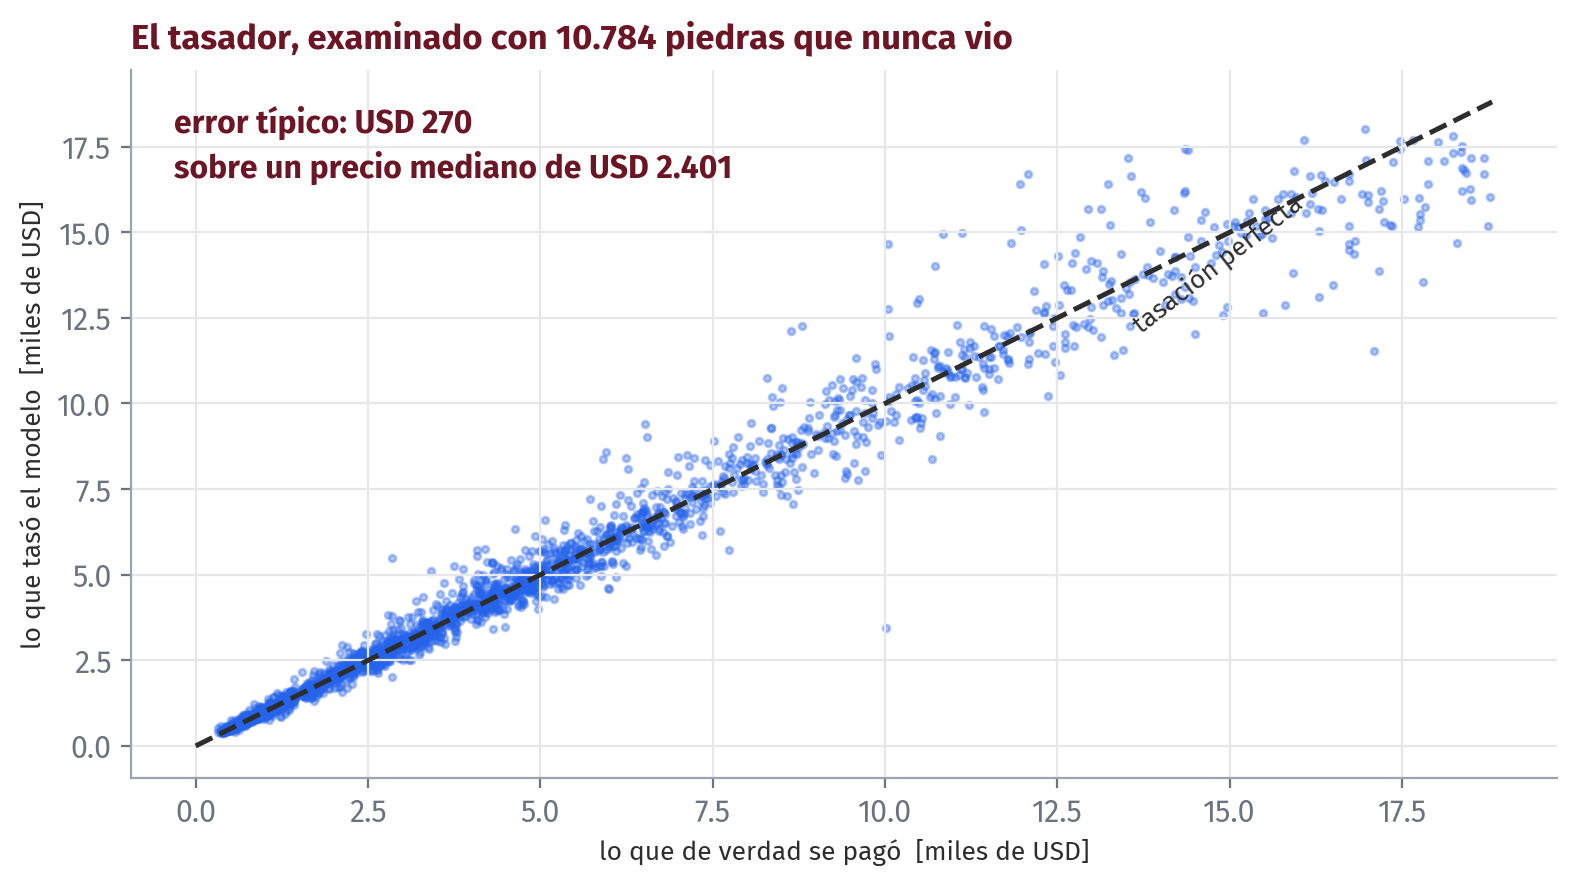
\includegraphics[width=0.82\textwidth, height=0.47\textheight, keepaspectratio]{fig_ajuste.png}\end{center}
  \vspace{2pt}
  {\footnotesize\color{textMuted}
   Entrenó en \textbf{2 segundos}. Error típico: \textbf{USD 270} sobre un
   precio mediano de \textbf{USD 2.401} --- alrededor de un 11\,\%. Para una
   mesa de compra que hoy tasa a ojo, eso ya es una herramienta.}
\end{frame}

\begin{frame}[shrink=8]{En Qué Se Fija --- y la Lectura Honesta}
  \vspace{-2pt}
  \begin{center}
\includegraphics[width=0.88\textwidth, height=0.44\textheight, keepaspectratio]{fig_importancias.png}\end{center}
  \vspace{2pt}
  {\footnotesize\color{textMuted}
   El ancho (45\,\%) y los quilates (43\,\%) dominan --- y \textbf{miden casi
   lo mismo}: el tamaño, contado dos veces. Estas barras dicen en qué se
   apoyó el modelo, \textbf{no qué causa el precio}. La distinción de
   siempre.}
\end{frame}
\begin{frame}[shrink=5]{El Error Silencioso: el Orden de las Columnas}
  \vspace{2pt}
  {\scriptsize\color{textMuted}
   El error más caro de servir modelos no lanza ningún mensaje. Es este:
   el modelo se entrenó con las columnas en un orden, y la app le arma la
   fila \textbf{en otro}.}
  \vspace{2pt}
  \begin{columns}[T]
    \begin{column}{0.47\textwidth}
      \begin{tcolorbox}[colback=arcaGray, colframe=codeGreen, boxrule=0pt,
        leftrule=3pt, arc=3pt, left=8pt, right=8pt, top=3pt, bottom=3pt]
        {\scriptsize\color{codeGreen}\bfseries SI PASA UNA TABLA CON NOMBRES}\\[2pt]
        {\scriptsize\color{textMuted}
         scikit-learn compara los nombres de las columnas contra los del
         entrenamiento y \textbf{reclama} si no cuadran. Protección gratis.}
      \end{tcolorbox}
    \end{column}
    \begin{column}{0.47\textwidth}
      \begin{tcolorbox}[colback=arcaGray, colframe=arcaRed, boxrule=0pt,
        leftrule=3pt, arc=3pt, left=8pt, right=8pt, top=3pt, bottom=3pt]
        {\scriptsize\color{arcaRed}\bfseries SI PASA NÚMEROS PELADOS}\\[2pt]
        {\scriptsize\color{textMuted}
         Nadie revisa nada: los quilates caen donde iba la profundidad, y
         la app tasa \textbf{basura con cara de precio}. Sin error, sin
         aviso.}
      \end{tcolorbox}
    \end{column}
  \end{columns}
  \vspace{2pt}
  {\scriptsize\color{arcaDark}\bfseries
   La versión general: el mundo del entrenamiento y el mundo de la app
   tienen que ser \textbf{idénticos} --- mismas columnas, mismo orden, misma
   preparación. Cuando difieren, el modelo que daba 98 en el cuaderno da
   basura en producción, y nadie sabe por qué.}
  \vspace{2pt}
  {\scriptsize\color{arcaDark}\itshape
   Este error tiene nombre en la industria y es una plaga. Ustedes ya saben
   cómo se ve --- y cómo se previene: la app le pasa al modelo una tabla con
   nombres, nunca números pelados.}
\end{frame}


% ═════════════════════════════════════════════════════════════════════════════
\sectionframe{Pasos 4 y 5 · Guardar y Servir}{El modelo es un archivo, y Gradio lo vuelve una herramienta \\[6pt] \normalsize 50 -- 72 min}
% ═════════════════════════════════════════════════════════════════════════════

\begin{frame}[fragile, shrink=5]{El Modelo Es un Archivo}
  \vspace{2pt}
  {\footnotesize\color{textMuted}
   Un modelo entrenado no vive en la sesión de Colab --- si se desconecta, se
   pierde y hay que reentrenar. Se \textbf{guarda como archivo}, igual que un
   documento:}
  \vspace{5pt}
  \begin{minted}[fontsize=\small, breaklines]{python}
import joblib

joblib.dump(tasador, "tasador_v1.joblib")   # guardar

tasador = joblib.load("tasador_v1.joblib")  # cargar
  \end{minted}
  \vspace{6pt}
  {\footnotesize\color{textMuted}
   Ese archivo \textbf{es} el producto del entrenamiento. Se versiona
   (\texttt{v1}, \texttt{v2}...), se comparte, y la app lo carga sin
   reentrenar nada.}
  \vspace{6pt}
  \begin{tcolorbox}[colback=arcaGray, colframe=arcaDark, boxrule=0pt,
    leftrule=3pt, arc=3pt, left=8pt, right=8pt, top=4pt, bottom=4pt]
    {\scriptsize\color{arcaDark}\bfseries
     Regla práctica en Colab: guárdenlo también en su Drive. La sesión se
     apaga; el Drive no.}
  \end{tcolorbox}
\end{frame}

\begin{frame}[shrink=8]{Gradio: Qué Es, y Por Qué Existe}
  \vspace{-6pt}
  \begin{columns}[T]
    \begin{column}{0.30\textwidth}
      \begin{center}
        
\includegraphics[width=0.52\linewidth]{_logos/gradio.png}\\[5pt]
        {\scriptsize\color{textMuted} desde 2021, parte de}\\[2pt]
        
\includegraphics[width=0.32\linewidth]{_logos/huggingface.png}\\[1pt]
        {\scriptsize\color{textMuted} Hugging Face}
      \end{center}
    \end{column}
    \begin{column}{0.66\textwidth}
      {\scriptsize\color{textMuted}
       Nació en \textbf{Stanford, en 2019}, por una frustración que les va a
       sonar: los investigadores tenían modelos médicos funcionando... y los
       \textbf{médicos} --- los que sabían si el modelo servía --- no podían
       probarlos sin pedirle una interfaz a un programador.
       \vspace{5pt}

       La solución fue radical: que \textbf{una función de Python se vuelva
       una página web} con controles, en una línea. Sin saber nada de
       páginas web.
       \vspace{5pt}

       Hoy es el \textbf{estándar de la industria} para poner un modelo en
       manos de alguien: las demos de IA más famosas de los últimos años
       corren sobre Gradio, y ya viene instalado en Colab.
       \vspace{5pt}

       \textbf{\color{arcaDark}Fíjense para quién se inventó: para que el
       experto de dominio tocara el modelo sin programar la interfaz. O sea:
       para ustedes.}}
    \end{column}
  \end{columns}
\end{frame}

\begin{frame}[shrink=5]{Y Qué Es el Link}
  \vspace{2pt}
  {\footnotesize\color{textMuted}
   Uno le dice \emph{«esta función recibe las medidas y devuelve el precio»},
   y Gradio arma solo la interfaz: las casillas, el botón, el espacio de la
   respuesta.
   \vspace{6pt}

   Y en Colab hace algo más: con \texttt{share=True} genera un \textbf{link
   público} --- una dirección que el comprador abre desde su celular en la
   mesa de compra, mientras el cuaderno de ustedes hace el trabajo por
   detrás. Es una extensión telefónica hacia su cuaderno, no una oficina
   nueva.}
  \vspace{7pt}
  \begin{tcolorbox}[colback=arcaGray, colframe=arcaRed, boxrule=0pt,
    leftrule=3pt, arc=3pt, left=9pt, right=9pt, top=5pt, bottom=5pt]
    {\scriptsize\color{arcaRed}\bfseries LO QUE HAY QUE SABER DEL LINK}\\[3pt]
    {\footnotesize\color{textMuted}
     Vive \textbf{mientras el cuaderno esté corriendo}. Si Colab se cierra o
     se desconecta, deja de responder. Perfecto para una demo o una jornada
     de trabajo; no es un sistema permanente --- eso se conversa en la
     Clase 3.}
  \end{tcolorbox}
\end{frame}

\begin{frame}[fragile, shrink=5]{Gradio en Tres Escalones · 1 y 2}
  \vspace{-2pt}
  {\scriptsize\color{textMuted}
   Antes del tasador, la anatomía en chiquito. \textbf{Escalón 1} --- toda
   app de Gradio son tres piezas: una función, sus entradas, sus salidas:}
  \vspace{2pt}
  \begin{minted}[fontsize=\scriptsize, breaklines]{python}
def saludar(nombre):
    return f"Hola, {nombre}"

gr.Interface(fn=saludar, inputs="text", outputs="text").launch()
  \end{minted}
  \vspace{3pt}
  {\scriptsize\color{textMuted}
   \textbf{Escalón 2} --- controles con tipo y unidades. El mismo patrón ya
   hace una herramienta de campo:}
  \vspace{2pt}
  \begin{minted}[fontsize=\scriptsize, breaklines]{python}
def a_metros_cubicos(barriles):
    return f"{barriles * 0.158987:,.1f} m3"

gr.Interface(fn=a_metros_cubicos,
             inputs=gr.Number(label="Barriles [bbl]", value=1000),
             outputs=gr.Textbox(label="Metros cúbicos")).launch()
  \end{minted}
  \vspace{2pt}
  {\scriptsize\color{arcaDark}\bfseries\itshape
   Función $\to$ entradas $\to$ salidas. El tasador es esto, con un modelo
   adentro.}
\end{frame}

\begin{frame}[fragile, shrink=5]{Gradio en Tres Escalones · 3: la Salida Es una Gráfica}
  \vspace{-2pt}
  {\scriptsize\color{textMuted}
   \textbf{Escalón 3} --- la salida no tiene que ser texto. Con
   \texttt{gr.Plot}, la función devuelve una figura --- y la app se vuelve
   un tablero:}
  \vspace{2pt}
  \begin{minted}[fontsize=\scriptsize, breaklines]{python}
def donde_cae(quilates):
    parecidas = d[abs(d.carat - quilates) < 0.1]
    fig, ax = plt.subplots(figsize=(7, 3))
    ax.hist(parecidas.price, bins=40)
    ax.set_xlabel("precio [USD]")
    ax.set_title(f"{len(parecidas)} piedras de ~{quilates} quilates")
    return fig

gr.Interface(fn=donde_cae,
             inputs=gr.Slider(0.2, 3.0, value=1.0, label="Quilates"),
             outputs=gr.Plot(label="Precios de piedras similares")).launch()
  \end{minted}
  \vspace{2pt}
  {\scriptsize\color{textMuted}
   Muevan el deslizador y la distribución cambia: la memoria de comparables,
   dibujada. \textbf{El tasador es el escalón 4.}}
\end{frame}

\begin{frame}[shrink=5]{El Encargo de la App}
  \vspace{2pt}
  \begin{prompt}[EL PROMPT DE LA DEMO --- el tasador, versión 1]
CONTEXTO: tengo `tasador` (RandomForest entrenado),
la lista `columnas` con el orden del entrenamiento,
y el DataFrame `d` certificado.

OBJETIVO: app de Gradio para la mesa de compra ---
quilates, corte, color, claridad y x, y, z como
entrada; el precio estimado en USD como salida.

RESTRICCIONES: controles en español con unidades;
corte, color y claridad como desplegables con los
valores de `d`; launch(share=True).

CRITERIO: tasar una piedra en menos de 30 segundos
sin ayuda.
  \end{prompt}
  \vspace{2pt}
  {\scriptsize\color{arcaDark}\itshape
   Detalle técnico que el agente debe resolver: la app recibe 7 valores,
   pero el modelo espera las columnas de \texttt{get\_dummies} en su orden.
   Si el agente no lo maneja, ahí está su primer error para cazar.}
\end{frame}

% ═════════════════════════════════════════════════════════════════════════════
\sectionframe{Paso 6 · Blindar}{El tasador funciona. Ahora, que no mienta \\[6pt] \normalsize 72 -- 90 min}
% ═════════════════════════════════════════════════════════════════════════════

\begin{frame}[shrink=8]{La Prueba que Nadie le Hace a su Propia App}
  \vspace{-2pt}
  \begin{center}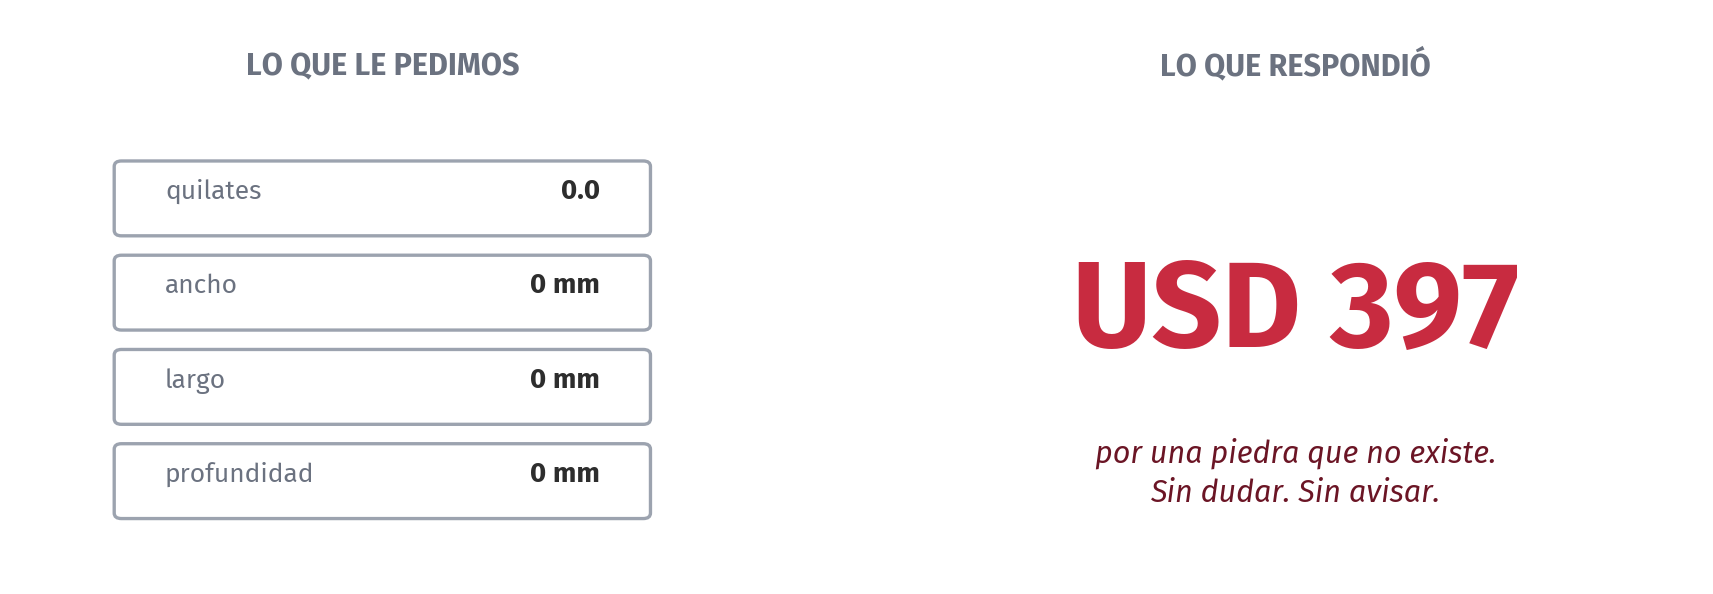
\includegraphics[width=0.94\textwidth, height=0.46\textheight, keepaspectratio]{fig_cero.png}\end{center}
  \vspace{2pt}
  {\footnotesize\color{textMuted}
   Le pedimos el precio de una piedra de \textbf{0 quilates y 0 milímetros}
   --- la misma clase de fila que rechazamos en el paso 1 --- y respondió
   \textbf{USD 397}. Sin dudar. Sin avisar.}
\end{frame}

\begin{frame}[shrink=5]{Por Qué Pasa, y Qué Es un Contrato}
  \vspace{2pt}
  {\footnotesize\color{textMuted}
   El modelo no sabe qué es un diamante. Sabe interpolar entre los casos que
   vio --- y si le dan un punto absurdo, interpola igual y devuelve un número
   con la misma cara de seguridad.}
  \vspace{5pt}
  \begin{tcolorbox}[colback=arcaGray, colframe=arcaRed, boxrule=0pt,
    leftrule=4pt, arc=3pt, left=9pt, right=9pt, top=6pt, bottom=6pt]
    {\footnotesize\color{arcaDark}\bfseries
     Un modelo servido sin contrato es un generador de basura con interfaz
     bonita.}
  \end{tcolorbox}
  \vspace{5pt}
  {\footnotesize\color{textMuted}
   El \textbf{contrato de entrada y salida} de una herramienta seria:
  \begin{itemize}\setlength{\itemsep}{3pt}
    \item[{\color{arcaRed}\scriptsize\faArrowRight}]
      \textbf{Entrada:} qué valores acepta, y en qué rangos. Los rangos no
      se inventan: salen \textbf{del dato certificado} (mínimos y máximos
      reales del entrenamiento).
    \item[{\color{arcaRed}\scriptsize\faArrowRight}]
      \textbf{Fuera de rango:} la app \textbf{no tasa} --- explica con un
      mensaje claro qué está mal.
    \item[{\color{arcaRed}\scriptsize\faArrowRight}]
      \textbf{Salida:} no un número seco --- un número \textbf{con banda},
      y con la advertencia si la piedra está cerca del borde de lo que el
      modelo conoce.
  \end{itemize}}
\end{frame}

\begin{frame}[shrink=8]{La Banda Sale Gratis: los 100 Árboles No Opinan lo Mismo}
  \vspace{-2pt}
  \begin{center}
\includegraphics[width=0.97\textwidth, height=0.44\textheight, keepaspectratio]{fig_banda.png}\end{center}
  \vspace{2pt}
  {\footnotesize\color{textMuted}
   Cada árbol del bosque da su tasación; la \textbf{discrepancia entre ellos
   es la banda} P10--P90 --- la misma idea de las bandas del Módulo 5, ahora
   dentro de una app. Y miren el panel izquierdo: a veces el precio real
   queda \textbf{fuera} de la banda. Así debe ser: promete el 80\,\%, no la
   certeza.}
\end{frame}

\begin{frame}[shrink=5]{El Encargo del Blindaje}
  \vspace{2pt}
  \begin{prompt}[EL PROMPT DE LA DEMO --- el tasador, versión 2]
Mejora la app del tasador con un CONTRATO de entrada
y salida:

ENTRADA:
- calcula los rangos válidos de carat, x, y, z DESDE
  el DataFrame certificado `d` (mínimo y máximo)
- si el usuario mete un valor fuera de rango, NO
  tases: muestra un mensaje claro que diga qué campo
  está mal y cuál es el rango aceptable

SALIDA:
- además del precio, la banda P10-P90 calculada con
  las predicciones de los árboles individuales
  (tasador.estimators_)
- formato: "USD 5.400 (banda: 4.900 a 6.100)"

CRITERIO DE ACEPTACIÓN:
- la piedra de 0 mm tiene que ser RECHAZADA con
  mensaje, no tasada
- una piedra normal se tasa igual que antes
  \end{prompt}
  \vspace{3pt}
  {\scriptsize\color{arcaDark}\itshape
   El criterio de aceptación es literalmente la prueba que la rompió. Así se
   blinda: cada error conocido se vuelve una prueba.}
\end{frame}

% ═════════════════════════════════════════════════════════════════════════════
\sectionframe{Su Turno · La Calculadora de Riesgo}{El mismo flujo, de punta a punta, hecho por ustedes \\[6pt] \normalsize 90 -- 115 min}
% ═════════════════════════════════════════════════════════════════════════════

\begin{frame}[shrink=5]{El Caso · La Aseguradora Marítima}
  \vspace{-2pt}
  \begin{columns}[T]
    \begin{column}{0.47\textwidth}
      \begin{tcolorbox}[colback=arcaGray, colframe=arcaRed, boxrule=0pt,
        leftrule=3pt, arc=3pt, left=7pt, right=7pt, top=3pt, bottom=3pt]
        {\scriptsize\color{arcaRed}\bfseries EL PROBLEMA}\\[2pt]
        {\scriptsize\color{textMuted}
         Su cliente asegura embarcaciones. Calibra su modelo de riesgo con
         el naufragio \textbf{mejor documentado}: los 891 pasajeros del
         Titanic.}
      \end{tcolorbox}
      \vspace{2pt}
      \begin{tcolorbox}[colback=arcaGray, colframe=arcaDark, boxrule=0pt,
        leftrule=3pt, arc=3pt, left=7pt, right=7pt, top=3pt, bottom=3pt]
        {\scriptsize\color{arcaDark}\bfseries LA DECISIÓN}\\[2pt]
        {\scriptsize\color{textMuted}
         Qué factores separaron a quienes sobrevivieron --- y cómo pesan
         en \textbf{protocolos} y en la \textbf{prima}.}
      \end{tcolorbox}
    \end{column}
    \begin{column}{0.47\textwidth}
      \begin{tcolorbox}[colback=arcaGray, colframe=arcaDark, boxrule=0pt,
        leftrule=3pt, arc=3pt, left=7pt, right=7pt, top=3pt, bottom=3pt]
        {\scriptsize\color{arcaDark}\bfseries EL COSTO DEL ERROR}\\[2pt]
        {\scriptsize\color{textMuted}
         Un modelo mal calibrado tarifica mal \textbf{todas} las pólizas a
         la vez.}
      \end{tcolorbox}
      \vspace{2pt}
      \begin{tcolorbox}[colback=arcaGray, colframe=codeGreen, boxrule=0pt,
        leftrule=3pt, arc=3pt, left=7pt, right=7pt, top=3pt, bottom=3pt]
        {\scriptsize\color{codeGreen}\bfseries QUÉ LES PIDIÓ}\\[2pt]
        {\scriptsize\color{textMuted}
         «La \textbf{calculadora de riesgo}: perfil del pasajero, y me da
         su probabilidad de sobrevivir. Con la seriedad del tasador.»}
      \end{tcolorbox}
    \end{column}
  \end{columns}
  \vspace{2pt}
  {\scriptsize\color{arcaDark}\bfseries
   Es \textbf{clasificación}, no regresión --- y el bosque también la sabe
   hacer.}
\end{frame}
\begin{frame}[shrink=5]{Desde Cero: Regresión y Clasificación}
  \vspace{2pt}
  {\footnotesize\color{textMuted}
   Hoy vieron la primera; su reto usa la segunda. Es la única diferencia
   entre la demo y lo que van a hacer:}
  \vspace{6pt}
  \begin{columns}[T]
    \begin{column}{0.47\textwidth}
      \begin{tcolorbox}[colback=arcaGray, colframe=arcaDark, boxrule=0pt,
        leftrule=3pt, arc=3pt, left=8pt, right=8pt, top=4pt, bottom=4pt]
        {\scriptsize\color{arcaDark}\bfseries REGRESIÓN --- la demo}\\[3pt]
        {\scriptsize\color{textMuted}
         La respuesta es un \textbf{número}: ¿cuánto vale?\\[3pt]
         \texttt{RandomForestRegressor}\\
         \texttt{.predict()} $\to$ USD 5.400}
      \end{tcolorbox}
    \end{column}
    \begin{column}{0.47\textwidth}
      \begin{tcolorbox}[colback=arcaGray, colframe=codeGreen, boxrule=0pt,
        leftrule=3pt, arc=3pt, left=8pt, right=8pt, top=4pt, bottom=4pt]
        {\scriptsize\color{codeGreen}\bfseries CLASIFICACIÓN --- su reto}\\[3pt]
        {\scriptsize\color{textMuted}
         La respuesta es un \textbf{sí o no}: ¿sobrevive?\\[3pt]
         \texttt{RandomForestClassifier}\\
         \texttt{.predict\_proba()} $\to$ 0,74}
      \end{tcolorbox}
    \end{column}
  \end{columns}
  \vspace{7pt}
  {\footnotesize\color{arcaDark}\bfseries
   Y el consejo profesional: entreguen la \textbf{probabilidad}
   (\texttt{predict\_proba}), no el veredicto. «74 de cada 100 como usted
   sobrevivieron» le sirve a una aseguradora; un «sí» seco, no.}
  \vspace{5pt}
  {\scriptsize\color{textMuted}\itshape
   Todo lo demás --- certificar, reservar el examen, guardar, servir,
   blindar --- es idéntico. Por eso el flujo es lo que se llevan, no el
   modelo.}
\end{frame}


\begin{frame}[shrink=5]{\faTools\hspace{4pt}Su Reto: los Mismos Seis Pasos \hfill {\normalsize\color{arcaRed}\faClock\hspace{4pt}25 min}}
  \vspace{-2pt}
  \begin{encargo}[SU ENCARGO --- dataset pasajeros\_titanic (891 filas, ya cargado en el cuaderno)]
    {\scriptsize\color{textMuted}
     El flujo completo, con sus propios prompts (la plantilla de la C1
     sirve en cada paso):\\[2pt]
     \textbf{1 Certificar:} faltantes, ceros, columnas sospechosas.\\[1pt]
     \textbf{2 Entrenar:} \texttt{RandomForestClassifier}, 20\,\%
     reservado antes.\\[1pt]
     \textbf{3 Examinar:} de cada 100 del examen, ¿a cuántos acierta?\\[1pt]
     \textbf{4 Guardar} con joblib.\quad
     \textbf{5 Servir:} Gradio con \texttt{predict\_proba}.\\[1pt]
     \textbf{6 Blindar:} rangos desde el dato; edad de 500 años, rechazada
     con mensaje.}
  \end{encargo}
  \vspace{2pt}
  \begin{tcolorbox}[colback=arcaGray, colframe=arcaRed, boxrule=0pt,
    leftrule=3pt, arc=3pt, left=8pt, right=8pt, top=3pt, bottom=3pt]
    {\scriptsize\color{arcaRed}\bfseries UNA ADVERTENCIA, SIN MÁS PISTAS}\\[2pt]
    {\scriptsize\color{textMuted}
     Si su modelo acierta \textbf{casi todo}, no celebren: \textbf{paren y
     desconfíen}. Algo en sus columnas huele --- encuéntrenlo.}
  \end{tcolorbox}
\end{frame}

\begin{frame}[shrink=5]{Puesta en Común}
  \vspace{2pt}
  {\footnotesize\color{textMuted}
   Entre mesas, cuatro preguntas:}
  \vspace{5pt}
  {\footnotesize\color{textMuted}
  \begin{itemize}\setlength{\itemsep}{6pt}
    \item[{\color{arcaRed}\scriptsize\faComments}]
      Al certificar: ¿qué encontraron --- cuántos faltantes, en qué
      columnas? ¿Qué decidieron hacer con la edad?
    \item[{\color{arcaRed}\scriptsize\faComments}]
      ¿Qué columnas le dieron al modelo, y \textbf{quién} eligió: ustedes en
      el prompt, o el agente por defecto?
    \item[{\color{arcaRed}\scriptsize\faComments}]
      ¿Qué acierto sacaron? ¿Alguna mesa sacó \textbf{casi 100 de 100}?
      --- que nos cuente qué columnas usó, y lo miramos juntos.
    \item[{\color{arcaRed}\scriptsize\faComments}]
      La calculadora: ¿devuelve un veredicto («sobrevive») o una
      \textbf{probabilidad}? ¿Cuál de las dos le sirve a una aseguradora?
  \end{itemize}}
  \vspace{6pt}
  {\footnotesize\color{arcaDark}\bfseries\itshape
   La tercera pregunta es la importante. Si nadie cayó, lo provocamos juntos
   --- porque en el trabajo real, esa trampa la van a pisar.}
\end{frame}

% ═════════════════════════════════════════════════════════════════════════════
\sectionframe{Cierre}{}
% ═════════════════════════════════════════════════════════════════════════════

\begin{frame}[shrink=8]{Lo Que Aprendimos Hoy}
  \vspace{-2pt}
  \begin{columns}[T]
    \begin{column}{0.48\textwidth}
      {\small\color{arcaDark}\bfseries\faLightbulb[regular]\hspace{5pt}Conceptos:}
      \vspace{4pt}
      {\footnotesize\color{textMuted}
      \begin{itemize}\setlength{\itemsep}{3pt}
        \item[{\color{codeGreen}\scriptsize\faCheck}]
          El \textbf{flujo completo}: certificar, entrenar, examinar,
          guardar, servir, blindar
        \item[{\color{codeGreen}\scriptsize\faCheck}]
          El examen con datos \textbf{reservados antes} de entrenar
        \item[{\color{codeGreen}\scriptsize\faCheck}]
          El error \textbf{en la unidad del negocio}: dólares, no
          R\textsuperscript{2}
        \item[{\color{codeGreen}\scriptsize\faCheck}]
          El \textbf{contrato} de entrada y salida
        \item[{\color{codeGreen}\scriptsize\faCheck}]
          La \textbf{banda} que sale de los árboles en desacuerdo
      \end{itemize}}
    \end{column}
    \begin{column}{0.48\textwidth}
      {\small\color{arcaDark}\bfseries\faTools\hspace{5pt}Herramientas:}
      \vspace{4pt}
      {\footnotesize\color{textMuted}
      \begin{itemize}\setlength{\itemsep}{3pt}
        \item[{\color{arcaRed}\scriptsize\faArrowRight}]
          \texttt{RandomForestRegressor} / \texttt{Classifier}
        \item[{\color{arcaRed}\scriptsize\faArrowRight}]
          \texttt{train\_test\_split} --- el 20\,\% reservado
        \item[{\color{arcaRed}\scriptsize\faArrowRight}]
          \texttt{joblib} --- el modelo como archivo
        \item[{\color{arcaRed}\scriptsize\faArrowRight}]
          \texttt{gradio} con \texttt{share=True} --- por fin, el link
      \end{itemize}}
      \vspace{5pt}
      \begin{tcolorbox}[colback=arcaGray, colframe=arcaRed, boxrule=0pt, leftrule=3pt,
        arc=3pt, left=6pt, right=6pt, top=4pt, bottom=4pt]
        {\scriptsize\color{arcaRed}\bfseries EL NÚMERO DEL DÍA}\\[3pt]
        {\scriptsize\color{textMuted}
         \textbf{USD 397.} Lo que el tasador sin contrato pagó por una
         piedra que no existe.}
      \end{tcolorbox}
    \end{column}
  \end{columns}
\end{frame}

\begin{frame}[shrink=5]{Los Resultados Negativos de Hoy}
  \vspace{4pt}
  {\footnotesize\color{textMuted}
   Como siempre, en voz alta:}
  \vspace{6pt}
  {\footnotesize\color{textMuted}
  \begin{enumerate}\setlength{\itemsep}{6pt}
    \item[{\color{arcaRed}\scriptsize\faTimes}]
      \textbf{El tasador tasó una piedra de 0 mm en USD 397}, con total
      confianza. Un modelo no sabe cuándo la pregunta es absurda; eso lo
      tiene que saber la app --- y la app la escriben ustedes.
    \item[{\color{arcaRed}\scriptsize\faTimes}]
      \textbf{La banda a veces no atrapa el precio real} --- lo vimos en la
      propia lámina. Promete el 80\,\%, y cumple el 80\,\%: la certeza no
      existe, y venderla sería mentir.
    \item[{\color{arcaRed}\scriptsize\faTimes}]
      Y el que hayan encontrado ustedes en el reto --- el modelo
      \textbf{demasiado bueno}. Lo que huele a perfecto, huele a trampa.
  \end{enumerate}}
  \vspace{7pt}
  \begin{tcolorbox}[colback=arcaGray, colframe=arcaDark, boxrule=0pt,
    leftrule=4pt, arc=3pt, left=10pt, right=10pt, top=6pt, bottom=6pt]
    {\footnotesize\color{arcaDark}\bfseries
     Los tres son la misma lección: el modelo hace números; el criterio de
     cuándo creerle sigue siendo de ustedes.}
  \end{tcolorbox}
\end{frame}

\begin{frame}[shrink=5]{Si Se Llevan Una Sola Cosa}
  \vspace{6pt}
  \begin{tcolorbox}[colback=arcaGray, colframe=arcaRed, boxrule=0pt, leftrule=4pt,
    arc=3pt, left=10pt, right=10pt, top=9pt, bottom=9pt]
    {\large\color{arcaDark}\bfseries
     Un modelo no es el producto. El producto es la herramienta que lo
     envuelve: certificada, examinada y blindada.}\\[6pt]
    {\footnotesize\color{textMuted}
     El modelo se entrenó en 2 segundos. Todo lo demás de la clase ---
     certificar el dato, reservar el examen, el contrato, la banda, los
     mensajes --- es lo que separa un juguete de una herramienta que alguien
     puede usar para decidir con plata.}
  \end{tcolorbox}
  \vspace{8pt}
  {\footnotesize\color{arcaDark}\itshape
   Y noten la proporción: 2 segundos de modelo, 2 horas de ingeniería
   alrededor. Esa proporción es la real en la industria.}
\end{frame}

\begin{frame}[shrink=5]{La Lista que se Llevan: los Seis Pasos, para SU Proyecto}
  \vspace{2pt}
  {\footnotesize\color{textMuted}
   Imprimible. Cada paso, con la pregunta que lo aprueba:}
  \vspace{5pt}
  {\footnotesize\color{textMuted}
  \begin{enumerate}\setlength{\itemsep}{5pt}
    \item \textbf{Certificar} --- ¿revisé ceros, faltantes e imposibles
          físicos, y escribí qué rechacé y por qué?
    \item \textbf{Entrenar} --- ¿reservé el examen \emph{antes}? ¿elegí yo
          las columnas, o las eligió el agente sin decirme?
    \item \textbf{Examinar} --- ¿tengo el error en la \emph{unidad del
          negocio}? ¿se lo puedo decir a mi jefe en una frase?
    \item \textbf{Guardar} --- ¿el modelo es un archivo con versión, o vive
          en una sesión de Colab que se va a apagar?
    \item \textbf{Servir} --- ¿alguien que no soy yo puede usarlo en 30
          segundos, desde un link?
    \item \textbf{Blindar} --- ¿la entrada absurda es rechazada con mensaje?
          ¿la salida lleva banda?
  \end{enumerate}}
  \vspace{6pt}
  \begin{tcolorbox}[colback=arcaGray, colframe=codeGreen, boxrule=0pt,
    leftrule=3pt, arc=3pt, left=8pt, right=8pt, top=4pt, bottom=4pt]
    {\scriptsize\color{textMuted}
     Seis preguntas con sí: proyecto entregable. Cualquier no: ya saben
     exactamente qué falta.}
  \end{tcolorbox}
\end{frame}

\begin{frame}[shrink=5]{Su Proyecto: Hoy Quedó la Pieza Central}
  \vspace{4pt}
  {\footnotesize\color{textMuted}
   Lo que hicieron hoy con el Titanic es \textbf{exactamente} lo que su
   proyecto necesita con su propio dato:}
  \vspace{6pt}
  {\footnotesize\color{textMuted}
  \begin{itemize}\setlength{\itemsep}{5pt}
    \item[{\color{codeGreen}\scriptsize\faCheck}]
      El flujo de seis pasos, con sus prompts
    \item[{\color{codeGreen}\scriptsize\faCheck}]
      La app con link --- el entregable
    \item[{\color{codeGreen}\scriptsize\faCheck}]
      Y seguramente ya cazaron \textbf{un error del agente} --- anótenlo,
      que es parte de la entrega
  \end{itemize}}
  \vspace{7pt}
  \begin{tcolorbox}[colback=arcaGray, colframe=codeGreen, boxrule=0pt, leftrule=3pt,
    arc=3pt, left=8pt, right=8pt, top=5pt, bottom=5pt]
    {\scriptsize\color{codeGreen}\bfseries\faCheck\hspace{4pt}PARA ESTA SEMANA}\\[3pt]
    {\scriptsize\color{textMuted}
     Entrega hasta el \textbf{jueves de la próxima semana}, equipos de hasta
     3. En la Clase 3: los peligros con nombre --- qué se puede pegar en un
     chat de IA y qué no, antes de que trabajen con datos de la empresa.}
  \end{tcolorbox}
\end{frame}

\begin{frame}[shrink=8]{Datos y Referencias}
  \vspace{4pt}
  {\footnotesize\color{textMuted}
  \begin{itemize}\setlength{\itemsep}{5pt}
    \item[{\color{arcaRed}\scriptsize\faDatabase}]
      \textbf{Datos:} \texttt{diamantes} (la demo) y
      \texttt{pasajeros\_titanic} (el reto), publicados en el repositorio
      del curso --- copias exactas de los conjuntos de práctica de seaborn.
    \item[{\color{arcaRed}\scriptsize\faBook}]
      \textbf{scikit-learn}, \textbf{joblib} y \textbf{Gradio}: las tres
      vienen instaladas en Colab.
    \item[{\color{arcaRed}\scriptsize\faFileCode}]
      Las figuras y \textbf{todas} las cifras de estas láminas salen de
      \texttt{figuras.py} con semilla fija. Las soluciones del reto
      \textbf{no existen en ningún archivo}: se construyen en clase.
  \end{itemize}}
  \vspace{7pt}
  {\scriptsize\color{arcaDark}\itshape
   Como siempre: corren el script y tiene que dar exactamente lo mismo. Si
   no da, es un error nuestro y queremos saberlo.}
\end{frame}

% ── GRACIAS ──────────────────────────────────────────────────────────────────
\begingroup
\setbeamertemplate{headline}{}
\setbeamertemplate{footline}{}
\setbeamertemplate{navigation symbols}{}
\begin{frame}[plain, noframenumbering]
  \begin{tikzpicture}[remember picture, overlay]
    \fill[arcaDark] (current page.south west) rectangle (current page.north east);
    \node[anchor=center, text=white, font=\Huge\bfseries]
      at ([yshift=1.5cm]current page.center) {¡Gracias!};
    \node[anchor=center, text=white!80, font=\large, text width=10cm, align=center]
      at ([yshift=0.2cm]current page.center)
      {Carlos Enrique Mosquera Trujillo};
    \node[anchor=center, text=white!60, font=\normalsize, text width=10cm, align=center]
      at ([yshift=-0.6cm]current page.center)
      {\faEnvelope\hspace{6pt}cmosquerat@unal.edu.co};
    \node[anchor=center, text=white!60, font=\normalsize, text width=11cm, align=center]
      at ([yshift=-1.3cm]current page.center)
      {Machine Learning for Petroleum Engineers Using Python};
    \node[anchor=center, text=white!40, font=\small]
      at ([yshift=-2.0cm]current page.center)
      {Módulo 7 · Clase 2 \quad$\cdot$\quad SLB Ecuador \quad$\cdot$\quad UDLA \quad$\cdot$\quad 2026};
  \end{tikzpicture}
\end{frame}
\endgroup

\end{document}
